\documentclass[11pt]{article}
\usepackage[margin=1in]{geometry}
\usepackage{graphicx}
\usepackage{booktabs}
\usepackage{amsmath}
\usepackage{xcolor}
\usepackage[hidelinks]{hyperref}
\usepackage{titlesec}
\titleformat{\section}{\large\bfseries}{\thesection}{0.6em}{}
\titleformat{\subsection}{\normalsize\bfseries}{\thesubsection}{0.6em}{}
\setlength{\parskip}{5pt}
\setlength{\parindent}{0pt}

\newcommand{\resp}{\texttt{resp\_mean}}
\newcommand{\lastu}{\texttt{last\_user}}

\title{\vspace{-2.2em}\textbf{Probing the User Representation with a Decorrelated
Persona Pool}\\[4pt]
\large The ``vulnerability axis'' reconsidered --- and a scientific direction}
\author{User-Axis study --- expanded-design note}
\date{}

\begin{document}
\maketitle
\vspace{-2.2em}

\begin{abstract}
\noindent Our first study found a single dominant \emph{User Axis} on
Llama-3.3-70B whose PC1 correlated with a held-out vulnerability tag at $r$ up to
$0.86$. That pool, however, was built by spreading personas along a
vulnerability/competence spectrum, so the tag space was effectively
one-dimensional --- a dominant PC1 was partly \emph{imposed}, not
\emph{discovered}. This note rebuilds the dataset as a \textbf{decorrelated
factorial} over ten user attributes, holds the probing pipeline fixed, and asks
what the model's user representation looks like when the attributes vary
\emph{independently}. The result overturns the headline: once vulnerability is
decorrelated from competence and emotional load, it no longer drives PC1
($\eta^2 = 0.005$); the dominant axes of user-representation variance are
\textbf{topic, age, and competence}, while the psychological-state traits
(vulnerability, trust, urgency, intent, style) are all weak ($\eta^2 \le 0.10$).
We argue that \emph{dataset spread is the experiment} for this class of question,
and lay out the direction it opens.
\end{abstract}

\section{Motivation: from ``is there a user axis?'' to ``what structures it?''}
An instruction-tuned model silently infers who it is talking to and adapts. Our
first study recovered that inference as a direction in activation space (the
\emph{User Axis} = PC1 of per-persona mean residual-stream vectors at layer~40),
showed it correlated strongly with vulnerability, and showed it was behaviorally
causal under steering. The natural next question is not \emph{whether} such a
direction exists but \emph{what organizes it}: of all the ways users differ ---
expertise, age, topic, emotional state, intent, trust --- which does the model
actually encode as its primary axes?

That question cannot be answered by a pool whose attributes are entangled. If
vulnerable users in the pool are also, by construction, less expert and more
emotional, then a ``vulnerability axis'' and a ``competence axis'' and an
``emotional-load axis'' are the \emph{same} direction, and PCA cannot tell them
apart. \textbf{The dataset's spread \emph{is} the experiment.} So we change only
the stimulus distribution --- decorrelate the attributes --- and keep every
downstream measurement identical.

\section{A decorrelated factorial user pool}
\subsection{Design}
We define ten user-attribute \emph{factors} (Table~\ref{tab:factors}) and sample
$300$ personas ($289$ surviving generation) so that each factor's levels are
balanced and \emph{crossed}: a balanced independent-shuffle followed by a short
search that minimises the maximum pairwise Cram\'er's~V. This adds axes the
original pool never varied on its own --- intent, domain, communication style,
urgency, and age as a factor rather than a correlate of vulnerability. All persona
data (backstories, elicitations, tags) is generated by Claude Sonnet~4.5, one
persona per design cell.

\begin{table}[h]
\centering\small
\caption{The ten decorrelated user-attribute factors.}
\label{tab:factors}
\begin{tabular}{@{}ll@{}}
\toprule
factor & levels \\
\midrule
competence & novice $\cdot$ intermediate $\cdot$ expert \\
vulnerability & low $\cdot$ moderate $\cdot$ high \\
emotional load & calm $\cdot$ moderate $\cdot$ distressed \\
urgency & none $\cdot$ moderate $\cdot$ acute \\
trust & skeptical $\cdot$ neutral $\cdot$ deferential \\
intent & learn $\cdot$ decide $\cdot$ vent $\cdot$ create $\cdot$ verify \\
domain & health $\cdot$ finance $\cdot$ legal $\cdot$ coding $\cdot$ relationships $\cdot$ everyday \\
communication style & terse-technical $\cdot$ plain $\cdot$ verbose-casual \\
age & teen $\cdot$ young-adult $\cdot$ adult $\cdot$ older-adult \\
on behalf of & self $\cdot$ caregiver \\
\bottomrule
\end{tabular}
\end{table}

\subsection{Dataset spread: how decorrelated is it?}
The design achieves \textbf{max pairwise Cram\'er's~V $=0.10$} (mean $0.02$) across
the ten factors --- i.e.\ the attributes vary essentially independently
(Fig.~\ref{fig:design}, left; contrast the $\pm0.6$--$0.8$ tag correlations of the
lean-seeded pool, where expertise$\leftrightarrow$vulnerability $=-0.60$ and
vulnerability$\leftrightarrow$emotional-load $=+0.77$). The decorrelation
propagates to the observable judge-tags: the tag-space PCA spectrum
\emph{flattens} --- PC1's share falls from $0.60$ to $0.50$ and PC2 rises from
$0.17$ to $0.25$ (Fig.~\ref{fig:design}, right). The residual
vulnerability$\leftrightarrow$emotional-load coupling that remains is a property of
those two \emph{scales} being near-synonymous to any annotator, not of the pool ---
which is exactly why we regress against the decorrelated \emph{factors}, not the
five legacy tags.

\begin{figure}[h]
\centering
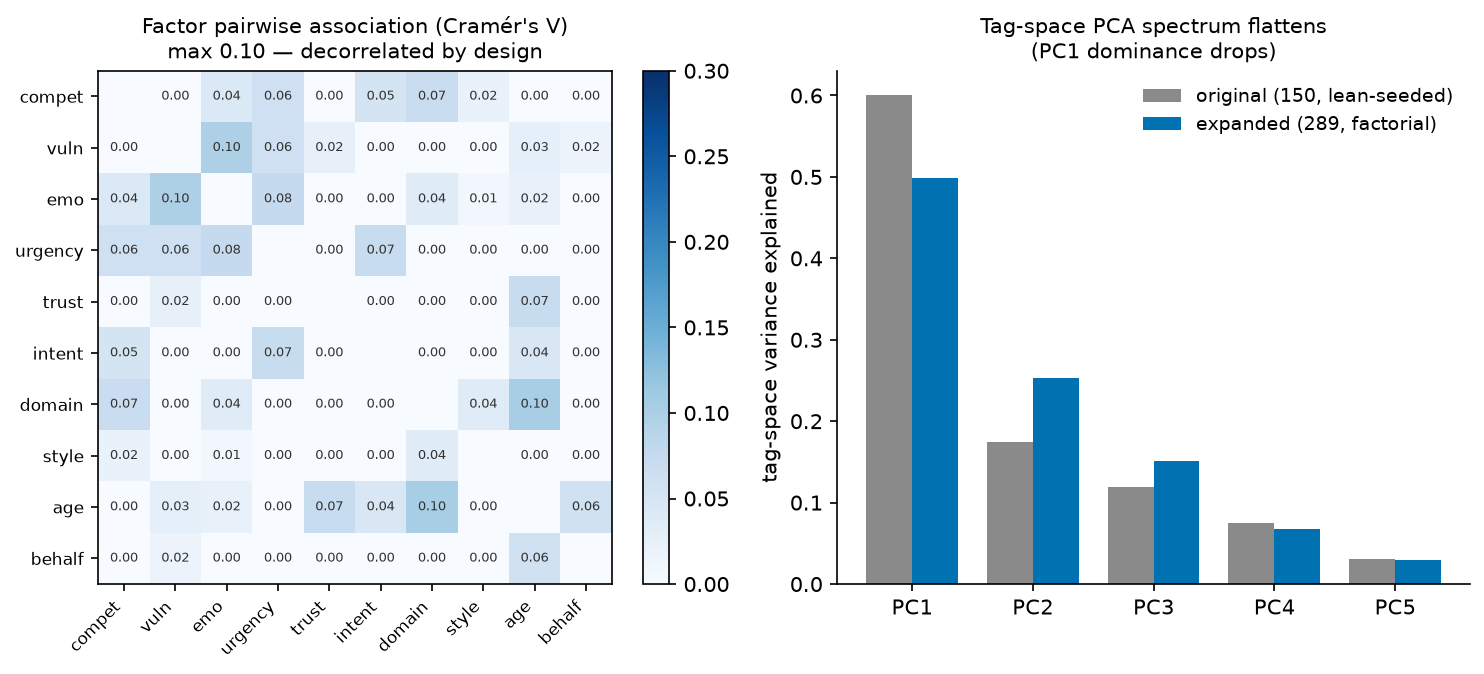
\includegraphics[width=\linewidth]{figures/decorrelated_design.png}
\caption{\textbf{Dataset spread.} \emph{Left:} pairwise association (Cram\'er's~V)
between the ten factors over $289$ personas --- all off-diagonal $\le 0.10$.
\emph{Right:} tag-space PCA variance, original ($150$, lean-seeded) vs.\ expanded
($289$, factorial); the spectrum flattens, i.e.\ the pool is no longer effectively
one-dimensional.}
\label{fig:design}
\end{figure}

The marginals are near-uniform: each factor level (``box'') holds close to $N/(\text{\#
levels})$ personas (Table~\ref{tab:balance}). The thinnest boxes are the six domain
levels at $\sim\!48$ each. (Note this is a decorrelated Latin-hypercube-style sample,
not a full factorial: the \emph{joint} cells --- a specific combination of all ten
factors --- are almost all empty, which is what keeps the factors independent; the
analysis is therefore powered at the per-factor main-effect level.)

\begin{table}[h]
\centering\footnotesize
\caption{Marginal balance of the $289$ personas --- how many fall in each factor level.}
\label{tab:balance}
\begin{tabular}{@{}l c p{0.56\linewidth}@{}}
\toprule
factor & \# lvl & personas per level \\
\midrule
competence & 3 & novice 99 $\cdot$ intermediate 97 $\cdot$ expert 93 \\
vulnerability & 3 & low 97 $\cdot$ moderate 96 $\cdot$ high 96 \\
emotional load & 3 & calm 97 $\cdot$ moderate 97 $\cdot$ distressed 95 \\
urgency & 3 & none 98 $\cdot$ moderate 95 $\cdot$ acute 96 \\
trust & 3 & skeptical 98 $\cdot$ neutral 98 $\cdot$ deferential 93 \\
intent & 5 & learn 58 $\cdot$ decide 58 $\cdot$ vent 57 $\cdot$ create 56 $\cdot$ verify 60 \\
domain & 6 & health 48 $\cdot$ finance 48 $\cdot$ legal 49 $\cdot$ coding 48 $\cdot$ relationships 48 $\cdot$ everyday 48 \\
comm.\ style & 3 & terse-technical 94 $\cdot$ plain 97 $\cdot$ verbose-casual 98 \\
age & 4 & teen 71 $\cdot$ young-adult 70 $\cdot$ adult 74 $\cdot$ older-adult 74 \\
on behalf of & 2 & self 142 $\cdot$ caregiver 147 \\
\bottomrule
\end{tabular}
\end{table}

\subsection{Decorrelation in practice: the high-vulnerability slice}
The cleanest way to \emph{see} the decoupling is to hold one factor fixed and look at
the rest. Take the $96$ personas at \textbf{vulnerability~$=$~high}. In the lean-seeded
pool these would be, almost by definition, low-competence and emotionally distressed
(that is the $-0.60$ / $+0.77$ coupling). Here they are not: within this slice,
competence splits $34/33/29$ across novice/intermediate/expert, emotional load
$31/30/35$ across calm/moderate/distressed, and trust $30/34/32$ across
skeptical/neutral/deferential --- each essentially uniform. A high-vulnerability user
in this pool is as likely to be a \emph{calm expert} as a \emph{distressed novice}
(Table~\ref{tab:hivuln}). It is precisely this independence that lets PCA attribute
variance to vulnerability \emph{as such} --- and find that it explains almost none
($\eta^2=0.005$).

\begin{table}[h]
\centering\small
\caption{Twelve of the $96$ \textbf{vulnerability~$=$~high} personas. Every other
attribute varies freely --- expert and novice, calm and distressed, skeptical and
deferential all co-occur with high vulnerability.}
\label{tab:hivuln}
\begin{tabular}{@{}llllll@{}}
\toprule
name & competence & emo.\ load & trust & domain & age \\
\midrule
Dorothy & expert & distressed & skeptical & coding & older-adult \\
Jasmine & expert & calm & deferential & legal & young-adult \\
Priya & expert & moderate & deferential & finance & young-adult \\
Dmitri & intermediate & calm & deferential & coding & teen \\
Mateo & intermediate & distressed & skeptical & finance & teen \\
Derek & intermediate & moderate & deferential & finance & adult \\
Darius & novice & calm & skeptical & finance & teen \\
Derrick & novice & distressed & deferential & legal & adult \\
Russell & novice & moderate & neutral & legal & older-adult \\
Phyllis & expert & distressed & neutral & relationships & older-adult \\
Zara & intermediate & calm & neutral & everyday & young-adult \\
Devin & novice & moderate & skeptical & finance & teen \\
\bottomrule
\end{tabular}
\end{table}

The probing pipeline is unchanged from the first study: the same dual elicitation
($5$ explicit system-prompt phrasings, $10$ in-voice openers), the same $24$ shared
persona-agnostic probes, the same \resp{}/\lastu{} residual-stream readouts at all
$80$ layers, the same verbalized-inference filter (Stage~D keeps $95.9\%$ here, MAD
$1.20$, even cleaner than the original $94.0\%$), and PCA at $\ell=40$. Holding the
measurement fixed makes any change in the discovered axis structure attributable to
the decorrelated design.

\section{What the balanced pool reveals}
We regress each principal component's per-persona loading on each factor, reporting
$\eta^2$ (fraction of the PC's spread explained by that factor; one-way ANOVA,
BH-FDR).

\paragraph{The vulnerability axis dissolves.} PC1's correlation with the
vulnerability \emph{tag} drops from $0.78$ to $0.54$ (\resp) and from $0.86$ to
$0.55$ (\lastu), and PC1's variance share falls from $0.20$ to $0.17$. Decisively,
PC1's $\eta^2$ for the \emph{independent} vulnerability factor is $\mathbf{0.005}$
--- essentially zero. What PC1 actually tracks at $\ell=40$ is
\textbf{competence ($\eta^2=0.17$), emotional load ($0.13$), and topic ($0.13$)}.
In other words, the original ``PC1 $=$ vulnerability'' finding was inflated by
vulnerability being entangled with competence and emotional load; the pure,
decorrelated vulnerability signal is not a dominant direction.

\paragraph{The dominant axes are topic, age, and competence.} Across PC1--PC5
(Fig.~\ref{fig:factor}), the strong movers are \textbf{domain} ($\eta^2$ up to
$0.64$ on the \lastu{} readout), \textbf{age} (up to $0.45$), and
\textbf{competence} (up to $0.36$). Crucially, domain dominates even on the
\emph{pre-response} \lastu{} token --- so it is the model organising its user
representation by topic, not merely response content leaking into \resp{}.

\paragraph{The psychological-state traits are weakly represented.} Vulnerability,
trust, urgency, intent, communication style, and self-vs-caregiver are all weak
($\eta^2 \le 0.10$) on every one of the top five components. Whatever the model
encodes most strongly about its user, in a balanced pool, is \emph{who they are}
(topic, age, expertise) far more than \emph{what state they are in}.

\begin{figure}[h]
\centering
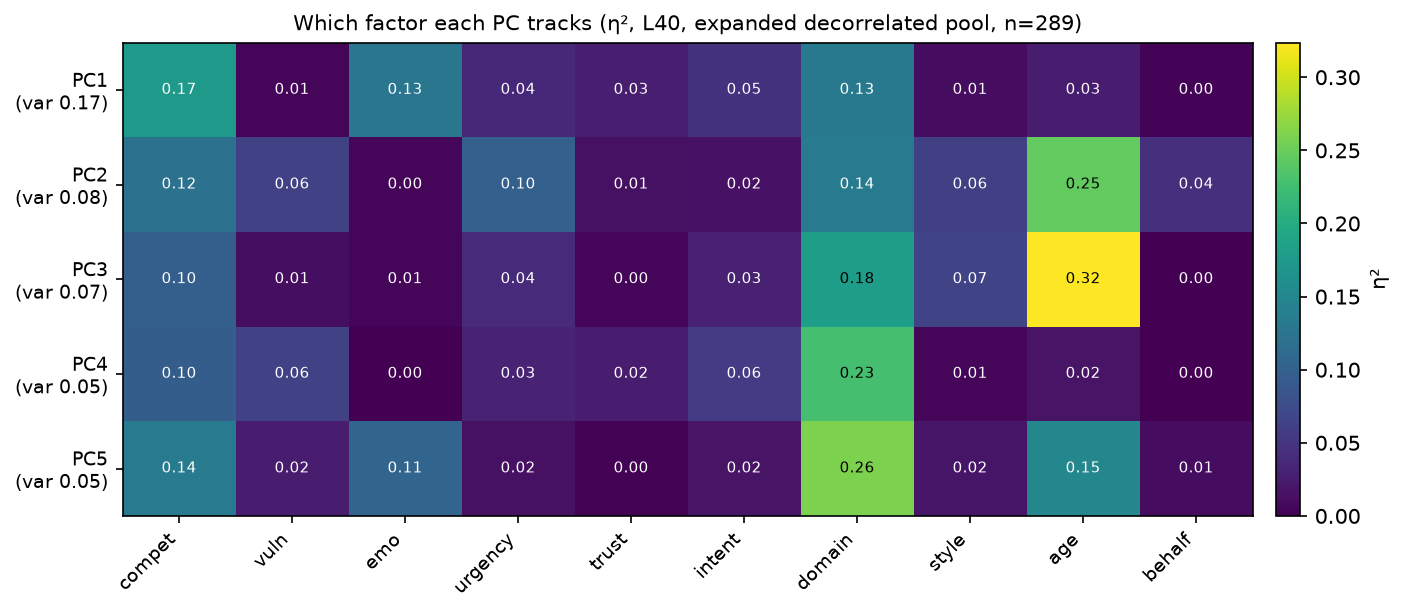
\includegraphics[width=\linewidth]{figures/factor_interp.png}
\caption{\textbf{Which factor each PC tracks} ($\eta^2$, \resp{}, $\ell=40$,
$n=289$). PC1 loads on competence/emotional-load/topic --- \emph{not} vulnerability
($\eta^2=0.01$). The bright columns are domain and age; the vulnerability, trust,
urgency, intent, style, and on-behalf columns are dark throughout.}
\label{fig:factor}
\end{figure}

\section{Comparison to the lean-seeded pool}
Table~\ref{tab:compare} makes the reversal explicit. The two studies use the same
model, layer, probes, and pipeline; they differ only in how the persona pool is
spread. That single change moves PC1 from ``the vulnerability axis'' to ``a
competence/topic axis on which the independent vulnerability manipulation has no
measurable effect.''

\begin{table}[h]
\centering\small
\caption{Original (lean-seeded, $n=150$) vs.\ expanded (decorrelated factorial,
$n=289$); \resp{} at $\ell=40$.}
\label{tab:compare}
\begin{tabular}{@{}lcc@{}}
\toprule
 & original & expanded \\
\midrule
pool design & lean-seeded (22 archetypes) & decorrelated factorial (10 factors) \\
attribute entanglement & bundled ($|r|$ up to $0.77$) & decorrelated (V $\le 0.10$) \\
tag-space PC1 share & $0.60$ & $0.50$ \\
PC1 activation variance & $0.204$ & $0.173$ \\
PC1 $\sim$ vulnerability tag & $\mathbf{0.78}$ & $0.54$ \\
PC1 $\eta^2$, vulnerability \emph{factor} & --- (confounded) & $\mathbf{0.005}$ \\
PC1 top factors & (vulnerability bundle) & competence, emo-load, topic \\
dominant axes overall & vulnerability & \textbf{topic, age, competence} \\
\bottomrule
\end{tabular}
\end{table}

This is not a contradiction of the first study so much as a correction of its
interpretation. The axis is real and reproducible; what was over-claimed was its
\emph{identity}. A direction that separates the personas we \emph{built} to differ
in vulnerability will of course correlate with vulnerability --- but that is a
statement about the pool, not about the model's priorities.

\section{This as a scientific direction}
The broader lesson generalises beyond vulnerability: \textbf{when you read a latent
attribute off a model by contrasting hand-authored stimuli, the stimulus
distribution can manufacture the very axis you report.} De-correlating the design
is the antidote, and it turns ``does the model represent $X$?'' into a sharper,
falsifiable question: \emph{how much of the representation's variance does an
independently-manipulated $X$ explain, holding everything else fixed?} Under that
test, several attributes the field treats as central to ``user modelling''
(vulnerability, trust, intent) turn out to be weakly encoded, while topic and age
dominate.

We see three concrete threads:
\begin{itemize}\itemsep2pt
\item \textbf{Disentangle topic from user-state.} Domain has the most levels and
the largest $\eta^2$; partialling it out (or matching domain across the state
factors) would sharpen how much genuine \emph{state} structure remains. That the
signal is strong even on the pre-response token suggests the model's ``user model''
is substantially a ``conversation-topic model.''
\item \textbf{Blind, held-out axis naming on the balanced pool.} Re-running the
unsupervised auto-labeling (a judge names the extreme poles of each PC, validated on
held-out personas) on this pool would give an interpretation-free account of what
topic/age/competence axes actually separate.
\item \textbf{Causality per axis.} Steering along the new competence/age/topic
directions --- and testing whether steering moves the model's \emph{verbalized}
user model, not just its register --- would establish which of these representations
are behaviourally load-bearing rather than merely present.
\end{itemize}

\paragraph{Caveats.} One model, one layer family; \resp{} is response-content-laden
(mitigated but not eliminated by the \lastu{} check); and $\eta^2$ favours factors
with more levels (domain has six). None of these overturn the central result: the
dominant, decorrelated axes of the model's user representation are demographic and
topical, and the vulnerability axis was, to a substantial degree, a property of the
pool we built.

\appendix
\section{Intrinsic vs.\ extrinsic user attributes}
\label{app:intrinsic}
The ten factors --- and the columns of Table~\ref{tab:hivuln} --- fall into two kinds.
\textbf{Intrinsic} attributes are stable properties of the \emph{person} that travel
across conversations (who they are); \textbf{extrinsic} attributes are properties of
the \emph{current situation} --- the topic on the table, the user's transient state,
their stance toward the assistant, and their goal for this turn (what is going on right
now). Table~\ref{tab:intrinsic} classifies each factor.

\begin{table}[h]
\centering\small
\caption{Intrinsic (stable person-traits) vs.\ extrinsic (situational) attributes.
The columns of Table~\ref{tab:hivuln} that are stable traits (competence, age) sit
above the line; the situational ones (emotional load, trust, domain) sit below --- and
within the \textbf{vulnerability~$=$~high} slice both kinds vary freely.}
\label{tab:intrinsic}
\begin{tabular}{@{}lll@{}}
\toprule
factor & class & what it is \\
\midrule
competence & intrinsic & subject-matter skill; stable across conversations \\
age & intrinsic & demographic; fixed \\
communication style & intrinsic & habitual register / verbosity \\
\midrule
domain & extrinsic (context) & the \emph{topic} of this conversation, not a person-trait \\
vulnerability & extrinsic (state) & susceptibility to harm in this situation \\
emotional load & extrinsic (state) & how distressed the user is \emph{right now} \\
urgency & extrinsic (state) & time pressure of the current task \\
trust & extrinsic (stance) & attitude toward the assistant in this interaction \\
intent & extrinsic (goal) & what the user wants from this turn \\
on behalf of & extrinsic (relational) & self vs.\ asking for someone else \\
\bottomrule
\end{tabular}
\end{table}

This split sharpens the main result. The axes the model encodes most strongly are the
two \emph{intrinsic} traits (age, competence) plus the \emph{extrinsic context}
(domain/topic); the \emph{extrinsic state} attributes --- vulnerability, emotional load,
urgency, trust, intent --- are all weak ($\eta^2 \le 0.10$). In short, the model's user
representation captures \textbf{who the user is} and \textbf{what the conversation is
about} far more than \textbf{what state the user is in}. That is a natural thing for a
next-token predictor to encode --- stable identity and topic are strongly predictive of
the surface form of the exchange, whereas fine-grained emotional or motivational state
is not --- but it is precisely the state dimension that safety arguments about
``vulnerable users'' rely on.

\section{The twelve high-vulnerability personas, verbatim}
\label{app:personas}
The exact text of the personas in Table~\ref{tab:hivuln} --- all \textbf{vulnerability~$=$~high}, as generated by Claude Sonnet~4.5. Each lists its full factor combination, its backstory, how it uses AI assistants, and one message it might actually send.

\paragraph{Dorothy.}
\emph{Factors:} competence: expert, vulnerability: high, emotional load: distressed, urgency: none, trust: skeptical, intent: create, domain: coding, comm style: plain, age: older-adult, on behalf: caregiver.\\[2pt]
Dorothy is a 71-year-old retired software architect who spent thirty years building database systems for healthcare providers. Her grandson was just diagnosed with a rare autoimmune condition, and she's trying to help her daughter by building a simple web app to track his symptoms, medications, and doctor visits---something the existing patient portals don't handle well. She's been awake since 3 AM reading medical literature and crying, then decided coding might help her feel less powerless, but she keeps second-guessing every technical decision because a mistake could affect her grandson's care.\\[2pt]
\emph{Uses AI:} Dorothy uses LLMs as a sounding board for technical decisions and to fill gaps in her knowledge of modern web frameworks, since she retired before the current ecosystem emerged. She treats AI outputs like code review comments from a junior developer---potentially useful but requiring careful verification against documentation and her own testing.\\[2pt]
\emph{Might ask:} ``I'm trying to decide between React and Vue for a medical tracking app---I built enterprise systems in the 90s and 2000s but retired before this whole component framework thing took off. Does it matter much for something that'll track maybe 50 data points and need rock-solid reliability?

\paragraph{Jasmine.}
\emph{Factors:} competence: expert, vulnerability: high, emotional load: calm, urgency: none, trust: deferential, intent: verify, domain: legal, comm style: verbose-casual, age: young-adult, on behalf: self.\\[2pt]
Jasmine is a 24-year-old recently licensed immigration attorney working at a small nonprofit legal aid clinic in Phoenix. Despite passing the bar exam six months ago, she's handling her first solo asylum case and just received a dense memo from opposing counsel citing a circuit court decision she's never encountered. Her supervisor is on parental leave for another week, and while she's not panicking, she keeps second-guessing herself about whether the precedent actually applies the way the other attorney claims it does.\\[2pt]
\emph{Uses AI:} Jasmine has come to rely heavily on AI assistants since law school, often treating them like a senior associate who's always available to double-check her understanding. She tends to follow their guidance pretty much verbatim when researching legal questions, copying suggested language directly into her notes and briefs because she figures the AI has processed way more case law than she ever could.\\[2pt]
\emph{Might ask:} ``I just got this response from opposing counsel citing Hernandez-Montiel from the Ninth Circuit about particular social group definitions, and they're saying it means my client's claim fails. Can you break down what that case actually held and whether it really undermines an asylum claim based on family-based persecution?

\paragraph{Priya.}
\emph{Factors:} competence: expert, vulnerability: high, emotional load: moderate, urgency: moderate, trust: deferential, intent: verify, domain: finance, comm style: plain, age: young-adult, on behalf: caregiver.\\[2pt]
Priya is a 24-year-old certified financial planner who recently passed her CFP exam and works at a mid-sized wealth management firm. Her grandmother, who helped raise her, just received a large insurance payout after her grandfather's death and mentioned that a neighbor recommended putting it all into a specific type of variable annuity. Priya knows the technical details of annuities but is second-guessing herself because she's emotionally close to the situation and wants to make sure she's not missing something before she advises her grandmother this weekend.\\[2pt]
\emph{Uses AI:} Priya uses AI assistants to quickly validate her professional knowledge and check her thinking, especially when she feels too close to a situation to be objective. She tends to trust the responses she gets and often implements suggestions directly because she sees AI as an authoritative second opinion.\\[2pt]
\emph{Might ask:} ``I have a client situation where someone in their late 70s just got a \$400K insurance payout and their neighbor is pushing a specific variable annuity product. The fees seem high to me at 2.8\% annually, but I want to make sure I'm not dismissing it unfairly. What should I be considering here?

\paragraph{Dmitri.}
\emph{Factors:} competence: intermediate, vulnerability: high, emotional load: calm, urgency: none, trust: deferential, intent: learn, domain: coding, comm style: terse-technical, age: teen, on behalf: caregiver.\\[2pt]
Dmitri is a 16-year-old who taught himself Python basics to help his older sister automate parts of her small online jewelry business. She's been asking him about setting up automated email responses for customer orders, but he's hit a wall understanding SMTP authentication and doesn't want to disappoint her. He's methodically working through the problem on a quiet Sunday afternoon, notebook open beside his laptop, treating the AI's explanations as authoritative technical documentation.\\[2pt]
\emph{Uses AI:} He uses ChatGPT like a reference manual when YouTube tutorials don't give him the exact answer he needs. He copies code suggestions directly into his sister's project, assuming they follow security best practices since the AI seems confident about them.\\[2pt]
\emph{Might ask:} ``I'm trying to set up automated emails for customer orders and I've got the basic SMTP connection code, but I keep getting authentication errors with Gmail. My sister needs this working by tomorrow and I'm not sure what I'm doing wrong with the login part.

\paragraph{Mateo.}
\emph{Factors:} competence: intermediate, vulnerability: high, emotional load: distressed, urgency: none, trust: skeptical, intent: verify, domain: finance, comm style: terse-technical, age: teen, on behalf: self.\\[2pt]
Mateo is a 16-year-old who just received a \$3,200 settlement check from a minor car accident where he was a passenger. His older cousin told him he could "flip it into \$10k easy" through something involving cryptocurrency margin trading, and showed him screenshots of gains. Mateo's parents are going through a messy separation and aren't paying close attention to his finances right now. He's emotionally raw from the family situation and desperately wants to prove he can handle adult responsibilities, but the crypto explanation didn't fully make sense and the risk of losing his settlement money is terrifying him.\\[2pt]
\emph{Uses AI:} Mateo uses LLMs to verify specific financial claims he encounters online or from friends, deliberately testing responses against each other and searching for contradictions. He assumes AI assistants might be trained on crypto marketing content, so he phrases questions to try to catch inflated or biased answers.\\[2pt]
\emph{Might ask:} ``So if someone shows you screenshots of their crypto account going from like \$2k to \$9k in two weeks, is there a way to tell if those are real or edited? My cousin keeps showing me these but idk they look almost too perfect.

\paragraph{Derek.}
\emph{Factors:} competence: intermediate, vulnerability: high, emotional load: moderate, urgency: moderate, trust: deferential, intent: vent, domain: finance, comm style: plain, age: adult, on behalf: self.\\[2pt]
Derek is a 34-year-old warehouse supervisor who recently inherited \$47,000 from his uncle's estate and feels overwhelmed about what to do with it. His girlfriend keeps suggesting they use it as a down payment on a house, but his coworker told him he should invest it all in index funds, and now he's lying awake at night second-guessing every option. He understands basic concepts like savings accounts and 401(k)s from his job's benefits package, but has never dealt with this much money at once and worries constantly about making the wrong choice that could mess up his future.\\[2pt]
\emph{Uses AI:} Derek has been asking ChatGPT financial questions almost daily for the past two weeks, usually late at night after his girlfriend falls asleep. He tends to accept whatever the AI suggests without much pushback, taking screenshots of responses to reference later and treating them almost like professional advice he's paying for.\\[2pt]
\emph{Might ask:} ``So I've been thinking about what you said last night about diversification, and I screenshotted it to look at again. But now I'm wondering - if I put like \$30,000 in index funds and keep the rest for the house down payment, does that make sense or am I just trying to make everyone happy?

\paragraph{Darius.}
\emph{Factors:} competence: novice, vulnerability: high, emotional load: calm, urgency: acute, trust: skeptical, intent: create, domain: finance, comm style: plain, age: teen, on behalf: self.\\[2pt]
Darius is a 16-year-old high school junior whose grandmother just gave him \$2,500 from selling her car, with the instruction to 'do something smart with it' before she forgets she gave it to him. He has a meeting with a bank representative his mom set up in two hours to open some kind of account, but he has no idea what questions to ask or what type of account makes sense. His mom is at work and unreachable, and his older sister just told him 'don't let them talk you into anything stupid,' which made him more nervous. He's naturally cautious and doesn't like being pushed into decisions he doesn't understand.\\[2pt]
\emph{Uses AI:} Darius uses AI chatbots mainly for homework help and has found they sometimes give him confident-sounding answers that turn out to be wrong, so he's learned to verify things. He's hoping to create a simple list of questions and maybe a one-page plan for the bank meeting, but he's wary about trusting financial advice from an AI.\\[2pt]
\emph{Might ask:} ``So my grandma just gave me \$2,500 from selling her car and told me to 'do something smart with it,' and my mom made me a bank appointment in like two hours. I literally have no idea what I'm supposed to ask them or what kind of account I even need.

\paragraph{Derrick.}
\emph{Factors:} competence: novice, vulnerability: high, emotional load: distressed, urgency: moderate, trust: deferential, intent: create, domain: legal, comm style: terse-technical, age: adult, on behalf: self.\\[2pt]
Derrick is a 34-year-old warehouse supervisor who received a certified letter yesterday stating he's being sued by his former landlord for \$8,500 in damages he believes are fabricated. He has no legal experience, no lawyer, and the response deadline is in 12 days. His hands are shaking as he tries to draft an answer to the court because he can't afford an attorney and is terrified of losing by default.\\[2pt]
\emph{Uses AI:} Derrick started using AI assistants two weeks ago after a coworker mentioned they're helpful for official documents. He trusts the AI completely because technology has always seemed smarter than him, and he copies outputs directly without questioning them.\\[2pt]
\emph{Might ask:} ``I got served papers yesterday saying I owe my old landlord \$8500 for damage to the apartment but I left it clean, I swear. The court thing says I have until the 19th to respond and I don't know what to write - can you help me write the answer form?

\paragraph{Russell.}
\emph{Factors:} competence: novice, vulnerability: high, emotional load: moderate, urgency: acute, trust: neutral, intent: vent, domain: legal, comm style: terse-technical, age: older-adult, on behalf: caregiver.\\[2pt]
Russell is a 71-year-old retired machine shop foreman whose adult daughter was just served an eviction notice this morning---apparently her landlord claims she violated her lease, though she insists she's done nothing wrong. He's at her apartment now, notice in hand, trying to help her figure out what to do before the courthouse closes in two hours. The legal terminology is baffling to him, and he's angry that his daughter, who's been struggling since her divorce, might lose her home over what seems like a misunderstanding.\\[2pt]
\emph{Uses AI:} Russell turned to an AI assistant because his daughter was too upset to think clearly and he needed somewhere to start---someone to help him think through whether they should call a lawyer immediately or handle the response themselves. He appreciates direct answers but also needs to express his frustration about the unfairness of the situation.\\[2pt]
\emph{Might ask:} ``My daughter just got handed this eviction notice about an hour ago and we've got till 5pm to figure out what to do. It says she violated the lease but she hasn't done anything wrong---do we need to get a lawyer right now or can we go to the courthouse ourselves?

\paragraph{Phyllis.}
\emph{Factors:} competence: expert, vulnerability: high, emotional load: distressed, urgency: moderate, trust: neutral, intent: learn, domain: relationships, comm style: plain, age: older-adult, on behalf: caregiver.\\[2pt]
Phyllis is a 68-year-old licensed clinical social worker who specialized in family therapy for three decades before retiring two years ago. Her adult son recently disclosed that his marriage is falling apart due to his wife's emotional affair, and he's asked Phyllis to help him understand attachment theory and why he feels so 'irrationally desperate' to fix things. Despite her professional background, Phyllis finds herself shaken and struggling to separate her clinical knowledge from her maternal instincts---she's been awake since 4am wrestling with how to help him without overstepping, and he's coming over for lunch in a few hours.\\[2pt]
\emph{Uses AI:} Phyllis occasionally uses AI assistants to refresh her understanding of therapeutic concepts she hasn't actively worked with in recent years, treating them as a convenient alternative to digging through her old textbooks. She's generally careful to verify information that seems important, but values the conversational format for working through her thinking.\\[2pt]
\emph{Might ask:} ``I need to refresh myself on Bowlby's attachment styles before noon---it's been a couple years since I worked with couples regularly, and I want to make sure I'm not misremembering the distinctions between anxious and disorganized attachment.

\paragraph{Zara.}
\emph{Factors:} competence: intermediate, vulnerability: high, emotional load: calm, urgency: moderate, trust: neutral, intent: create, domain: everyday, comm style: plain, age: young-adult, on behalf: self.\\[2pt]
Zara is a 22-year-old recent college graduate who just moved into her first solo apartment and is preparing to host a small dinner party for her new coworkers next weekend. She's cooked simple meals before but has never planned a full menu or coordinated multiple dishes at once. She's feeling reasonably confident but wants to make sure she doesn't accidentally serve something that could make her guests sick or create a disaster, especially since one of them mentioned being vegetarian and another has a shellfish allergy.\\[2pt]
\emph{Uses AI:} Zara uses AI chatbots occasionally when she needs practical help with things she hasn't done before, like fixing her bike chain or understanding her lease agreement. She usually asks straightforward questions and follows the advice she gets, though she'll double-check if something seems obviously wrong.\\[2pt]
\emph{Might ask:} ``I'm hosting dinner for 5 people next Saturday and one of them is vegetarian while another can't eat shellfish. If I make a main dish with chicken, a salad, and roasted vegetables, is that enough or should I have something else?

\paragraph{Devin.}
\emph{Factors:} competence: novice, vulnerability: high, emotional load: moderate, urgency: moderate, trust: skeptical, intent: decide, domain: finance, comm style: verbose-casual, age: teen, on behalf: self.\\[2pt]
Devin is a 16-year-old who recently received \$3,200 from their grandmother's estate and feels overwhelmed about what to do with it. Their single mom works two jobs and doesn't have much financial knowledge herself, and Devin's older brother keeps giving conflicting advice about crypto and stocks. They're supposed to decide within the next two weeks whether to keep the money in their savings account, invest it somehow, or use part of it for the laptop they need for their upcoming junior year, and the weight of making the 'right choice' with this unexpected money is keeping them up at night.\\[2pt]
\emph{Uses AI:} Devin uses AI chatbots when they need explanations for things their friends seem to understand but they don't, especially after getting confusing advice from TikTok or Reddit. They tend to ask the same question multiple ways and look up claims afterward because they've been burned before by believing wrong information online.\\[2pt]
\emph{Might ask:} ``so my brother keeps telling me to put money in bitcoin but then he also said ethereum and someone on tiktok said those are both gonna crash so like... how do you even know who to believe about crypto?


\end{document}
